\chapter{绪论}

\section{研究背景及意义}

区块链(Blockchain)是一种按照时间顺序将数据区块以链条的方式组成的特定数据结构,被视为一个分布式的共享账本和数据库。它能够使用户无需相互信任与可信第三方的条件下完成可信的价值传输\cite{SurveyofEnterpriseBlockchains}。作为区块链2.0 的以太坊\footnotemark[1]\footnotetext[1]{\href{http://github.com/ethereum/wiki/wiki/White-Paper/}{以太坊白皮书}}重新将智能合约描述为图灵完备的、部署于区块链网络中合同条款代码。这意味着传统的合同条款可以进入实体计算机中,且在区块链网络去中心化、不可伪造、不可篡改的特性下严格执行。区块链推进了人与企业之间和线上与线下之间的全方面互联,其被成为下一代的新型生产关系。随着区块链的快速发展, 智能合约极大地丰富和扩展了区块链应用场景。它们为供应链、金融等传统领域带来重大变革, 已经快速渗入到人们生活的方方面面。

当前, 区块链分为公有区块链、联盟区块链和私有区块链。如表\ref{blockchain_type}所示, 公有链没有准入限制, 没有监管方可以组织参与, 任何人都可以参与共识, 常见的两种共识协议为工作量证明机制(Proof of work, 简称PoW)和权益证明机制(Proof of stake, 简称PoS)。由于任何人都可以自由加入, 因此公有链网络具有高度分布式的拓扑结构。但是, 公有链在安全性和性能方面也进行了权衡。公有链上的许多服务器遇到了扩展瓶颈, 吞吐量相对较弱; 与公有区块链的无准入限制形成鲜明对比的是, 私有区块链建立了准入规则, 规定谁可以查看和写入区块链。因为在控制方面有明确的层次结构, 私有链也不是去中心化系统。在某些私有链中, 具备安全模型的背景下,共识协议是多余的。因此在私有区块链中,不使用PoW并不会造成很严重的威胁, 因为每个参与者的身份都是已知的, 是手动进行管理的; 联盟区块链是介于公有链和私有链之间的,结合了两者的特征要素。在共识方面, 联盟链将少数同等权力的参与方视为验证者,而不是像公有链那样开放的系统, 让任何人都可以验证区块, 也不是像私有链那样, 通过一个封闭的系统, 只允许某一个实体来任命区块的生产者。对于从事各类活动的个人和企业来说,存在大量的区块链选择。即使在公有链、私有链和联盟链中,根据复杂性的不同,也会出现许多不同的用户体验。根据实际使用情况,企业可以选择最适合实现自己目标的产品。供应链、电商、医疗等需要彼此之间需要相互沟通的场景下, 联盟链可减轻私有链中交易对手的风险, 并且较少的节点数通常可使它们能够比公共链更有效率的运行, 通常选择联盟链作为企业级区块链的底层。

{\footnotesize
\begin{longtable}[h]{m{70pt}|m{70pt}|m{70pt}|m{70pt}}
    \caption[区块链类型]{区块链类型} \label{blockchain_type} \\
        \hline  
        &公有区块链&私有区块链&联盟区块链\\
        \hline
        准入限制&无&有&有\\
        \hline
        读取者&任何人&仅限受邀用户&相关联用户\\
        \hline
        写入者&任何人&获批参与者&获批参与者\\
        \hline
        所属者&无&单一实体&多方实体\\
        \hline
        交易速度&慢&快&快\\
        \hline
    \end{longtable}
}

与此同时, 云原生(Cloud Native)作为一种基于云的基础之上的软件架构思想,以及基于云进行软件开发实践的一组方法论。因其弹性和分布式的优势成为当今流行的软件服务模式。区块链即服务(Blockchain as a Service, 简称BaaS)则是基于云的一种构建、管理、托管和运维区块链网络及其应用的云服务平台\cite{onik2019performance}。BaaS支持将任何企业级区块链实施到云环境,而无需任何IT专业知识。这大大降低了区块链技术的使用门槛, 是促使区块链技术更广泛、更深入地渗透到各个行业和企业的催化剂, 其市值预计从2018年的6.23亿美元猛增2023年的150亿美元\footnotemark[1]\footnotetext[1]{\href{https://www.reportbuyer.com/product/5486837/global-blockchain-as-a-service-market.html}{Global Blockchain-as-a-Service Market 2018-2022}}。其中, 云厂商提供了大多数的BaaS平台\cite{KuernetesbasedFabricChaincodeManagementAndHihgAvailabilityTechnology}, 如表\ref{major_BaaS_platforms}所示, 其底层区块链支撑技术大多数选择IBM开源的跨企业级联盟链Hyperledger Fabric, 这也是本文选择Hyperledger Fabric的原因。

{\footnotesize
\begin{longtable}[h]{m{150pt}|m{200pt}}
    \caption[主要公有云的BaaS平台]{主要公有云的BaaS平台} \label{major_BaaS_platforms} \\
        \hline  
        BaaS平台&区块链平台\\
        \hline
        AWS区块链服务&Hyperledger Fabric, Ethereum\\
        \hline
        Azure区块链服务&Ethereum\\
        \hline
        Google Cloud Platform&不支持\\
        \hline
        IBM区块链服务&Hyperledger Fabric\\
        \hline
        阿里云区块链服务&Hyperledger Fabric, 蚂蚁区块链, Ethereum\\
        \hline
        腾讯云区块链服务TBaaS&Hyperledger Fabric, FISCO BCOS, Tencent TrustSQL\\
        \hline
        华为云区块链服务BCS&Hyperledger Fabric\\
        \hline
    \end{longtable}
}

% 挑战
然而, 当前BaaS平台的发展尤其是底层的区块链基础设施的建设依旧存在诸多挑战。
第一, 基础商业化应用工具并不完善\footnotemark[1]\footnotetext[1]{\href{http://www.caict.ac.cn/kxyj/qwfb/ztbg/202107/P020210726503897354430.pdf}{区块链基础设施研究报告(2021年)}}。虽然市场上存在多种可选择的BaaS平台解决方案, 但是这些BaaS平台由商业巨头把控, 行业马太效应明显\cite{KuernetesbasedFabricChaincodeManagementAndHihgAvailabilityTechnology}。BaaS平台的构建需要专业的区块链以及云原生的技术能力, 只有实力雄厚的云厂商进行BaaS平台的研发, 这些BaaS服务往往与云计算节点捆绑, 用户租用BaaS服务计费高昂, 这并不利于中小型企业构建自身私有BaaS平台以及区块链应用。
第二, 现阶段BaaS平台利用云能力对区块链基础设施赋能乏力。对于BaaS平台市场规模的不断膨胀, 需要找到解决当前区块链网络部署、备份、升级以及数据存储以及可扩展性的方法。然而当前BaaS平台仅提供了一种基于开源区块链平台的一键化自动部署管理方案, 未深入到区块链与云基础设施的底层。这并不是有效的云化方式, 浪费了云原生技术的潜力。

% 意义、愿景
针对上述问题, 本文选择面向联盟链场景开源框架Hyperledger Fabric和Kubernetes构建BaaS平台的区块链基础设施。通过对Hyperledger Fabric的ca、peer、orderer组件进行抽象适配使其更原生的运行于Kubernetes。

本课题拟实现Hyperledger Fabric Operator能够对fabric网络进行主动的持续管理,包括故障转移、备份、升级和自动缩放,使用户通过专家提供的知识获得类似云的自我管理。具体一点就是,如果我们采用Blockchain Automation Framework发布了一个POD,然后我们在K8S中误删了POD,那么其是不会替我们自动重建POD的,这是该项目的的主要问题所在。

为解决上述挑战, 本文
Hyperledger Fabric Operator: 云原生时代下Fabric管理工具
利用Kubernetes,72\%的工程师在云原生生产中使用Kubernetes[3],可以方便的迁移到支持Kubernetes的任何云 
更简单、更原生的: 使用kubectl命令管理Fabric, 显示于k8s-dashboard;复用Kubernetes, API公共功能如CRUD、watch、内置认证
管理Fabric: 声明式自动化配置静态组件,如: CA、HF网络组件.命令式创建动态通道、链码

由linux基金会牵头,包括 IBM等30家初始企业成员共同成立的Hyperledger Fabric项目成为流行的面向联盟链场景开源框架之一。该项目定位是面向企业的分布式账本平台,引入权限管理,设计上支持可插拔、可扩展,自开源依赖广受欢迎,github上已经有12.7k star。然而云原生时代下,Fabric缺乏一个成熟的、一站式的解决方案来解决在云计算平台上构建区块链联盟链(私有链)。即区块链如何和云计算快速深度结合,利用云计算伸缩性、可移植性和高可用性价值来提供“高质量”的区块链服务,是当前仍然遗留的挑战。


为了解决上述挑战,本文提出了一种面向领域驱动设计的战术建模支持方法及工具,
具体工作内容如图\ref{workresult}所示。
战术建模方法包括一套标准化的\textbf{战术建模指南},
用于帮助理解不同模式的特征属性、
使用时机以及实现技术,作为领域建模的理论支撑指导建模过程;
根据战术建模指南,本文还基于UML的profile扩展机制实例化\textbf{战术建模语言},
用于规范化使用战术建模模式进行领域建模的流程;
基于所提出的战术建模方法,本文还实现了一种\textbf{战术建模支持工具},
支持可视化建模、验证建模结果以及存储和扩展建模结果,
为战术建模支持方法提供可视化方式展现。


\begin{figure}[h] %figure环境,h默认参数是可以浮动,不是固定在当前位置。如果要不浮动,你就可以使用大写float宏包的H参数,固定图片在当前位置,禁止浮动。
    \centering %使图片居中显示
    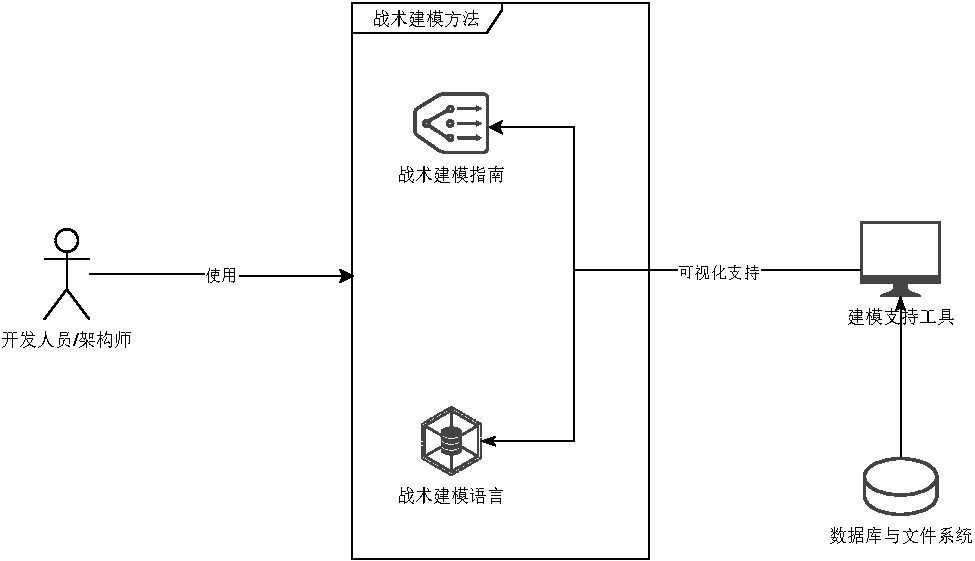
\includegraphics[width=0.8\textwidth]{FIGs/chapter1/workresult.pdf} %中括号中的参数是设置图片充满文档的大小,你也可以使用小数来缩小图片的尺寸。
    \caption{战术建方法及支持工具} %caption是用来给图片加上图题的
    \label{workresult} %这是添加标签,方便在文章中引用图片。
\end{figure}%figure环境



\section{国内外研究现状}

云原生背景下的区块链自诞生以来就受到了学术界与工业界的广泛关注。在区块链与云原生深度结合方面都进行了积极的探索。

% 学术
基于 Kubernetes 的 Fabric 链码管理及高可用技术[5]
(1)比较全面地研究了底层基础设施,尤其是生产环境下的高可用性 Kubernetes 平台
(2)设计并实现了Fabric在 Kubernetes上的云化部署,尤其是链码部分通过一个全新的容器控制插件实现了对 Kubernetes在代码级别上的支持,并完成了将链码纳入 Kubernetes环境管理的目标
云化的链码管理局限在链码层面, 无法实现对fabric网络进行主动的持续管理,包括故障转移、备份、升级和自动缩放

% 工业界
 Cello[6]: 一个区块链供应和操作系统,帮助人们以更高效的方式使用和管理区块链。Cello基于先进的区块链技术和现代PaaS工具,提供以下主要功能:
(1)管理区块链网络的生命周期
(2)支持自定义区块链网络配置,如网络大小、共识类型。
(3)支持多种底层基础设施,包括裸机、虚拟机、vSphere、本机Docker主机、swarm和Kubernetes
Cello当前阶段重点关注在Docker安装, 对Kubernetes operator支持方面的仍处在相对初级阶段,配置项简单灵活性不足且老旧,对CRD的最新更新在2年前;缺少对Operator的监控

Blockchain Automation Framework利用Ansible、Helm和Kubernetes部署生产DLT(分布式记账)网络。具体来说,使用helm charts作为Kubernetes部署模板、利用Ansible对网络进行配置。Blockchain Automation Framework框架目前支持Corda、Hyperledger Fabric、Hyperledger Indy和Quorum。然而,该项目采用的Ansible-Playbooks配置部署。本质上还是描述为一个需要希望远程主机执行命令的方案,或者一组IT程序运行的命令集合。虽然采用执行命令脚本的方式大大提升了自动化程度,但其远没有发挥k8s的潜力。

% 总结


领域驱动设计自提出以来,受到了学术界与工业界的广泛关注。
战略建模层次的实践与实现代码关联不紧密,更多关注的是顶层设计与架构搭建,
实施者一般也拥有较多的开发经验与较高的建模水平,所以在国内外都能较好地进行落地。
但战术建模层次更加侧重于建模的设计过程和具体实现,
对于建模实施者的水平有较高的要求,
还需要通过统一标准化的流程来达到建模结果的准确性,
规范化的建模语言也是支持战术建模成功实施的必要条件。所以,
一套完整的战术建模支持方法及工具就显得格外重要。

特定领域建模语言(Domain Specific Modeling Language)\cite{{frank2013domain}}
是一种专注于某个特定领域,结合了特定领域知识和概念的建模语言。
可以使用特定领域建模语言来进行战术建模,
从而获得统一标准化且具有特定领域特征的建模结果。
目前国内外研究人员对特定领域建模语言的定义方法了一些研究。
Hao Wu等人\cite{wu2018workflow}指出,
可以通过UML结合对象约束语言(Object Constraint Language,OCL)
的方式来扩充医疗系统领域现有元模型,形成一种更为完整的建模语言及方法。
Kühlwein等人\cite{kuhlwein2019firmware}通过一种分层架构的思想来打通物联网领域的多种元模型,
构建了一种平台型的特定领域建模语言,其中每层都有针对不同设备的元模型,
通过该平台进行组织和交互,这种定义方法需要依赖较为成熟的元模型;
Jumagaliyev等人\cite{jumagaliyev2019modelling}通过对云存储平台的通用存储类型进行分析,
抽象出数据类型的特征属性,创建元模型并使用EuGENia\cite{kolovos2010epsilon}进行注释,
最终借助Eclipse IDE将创建的元模型转换为具体的图形建模框架编辑器,
不仅定义了特定于云存储平台的元模型,还提供了建模工具编辑器。

国内外研究人员也对领域驱动设计建模语言的定义进行了一些研究。
Florian Rademacher等人\cite{rademacher2017towards}根据领域驱动设计实践经验提出使用UML profile
定义元模型,并将其应用到微服务领域中去。
Florian Rademacher等人调研了大量领域建模的UML图,
确定了可以描述领域模型的UML类图的构造方法。通过扩展元类的方式,
达到了使用领域驱动设计战术建模实现微服务系统建模的目的,
并为验证模型有效性和实现微服务代码奠定了基础。
同样的,Hippchen等人\cite{hippchen2019systematic}也强调了微服务化拆分中应用面向领域驱动设计建模语言的好处。
Florian Rademacher等人强调了领域驱动设计概念在UML中缺少正式的定义,阻碍了模型的验证和转化,
但同时UML又符合软件设计领域建模的要求,应用也十分广泛,故以UML为基础进行扩展,
定义出了一套新的针对领域驱动设计相关规则和约束的建模语言。
Andreas Diepenbrock等人\cite{diepenbrock2017ontology}提出使用本体论(Ontology)\cite{smith2003ontology}
来定义针对微服务应用的领域驱动设计元模型,该研究主要使用了本体论在特定领域表达知识语义的功能,
结合领域驱动设计实现了建模的目的。

以上工作说明任何特定领域建模语言的定义与提出都需要前期大量领域实践知识的总结,
并且在已有工作成果的基础上进行元模型的定义效率更高。
由于领域驱动设计战术建模理论较为成熟,
目前定义的战术模式特征明确,所以,
本文将基于领域驱动设计战术建模的现有研究成果,
结合实际应用情况,进行修改和优化,
定义一套新的领域驱动设计战术建模语言。


除了定义元模型来实现建模语言之外,提供支持建模语言的工具也十分重要。
刘辉等人\cite{刘辉2008元建模技术研究进展}提出元建模工具的实现主要分为两种途径。
第一种是使用配置文件扩展通用建模工具,让通用建模工具支持特定领域的元模型从而支持特定领域建模语言。
Guerriero等人\cite{guerriero2018streamgen}通过UML的profile扩展机制,
扩展了现有UML的语法元模型,达到创建新的元模型的目的,
扩展UML语法元模型的实现方式只依赖于配置文档,有利于多种建模方法的集成,
但需要借助统一建模语言的实现平台,如MetaEdit+\footnotemark[3]\footnotetext[3]{MetaEdit+首页:https://www.metacase.com/products.html}。
第二种是通过建模工具生成器根据元模型直接生成相应的建模工具,
La Fosse等人\cite{la2019towards}使用GEMOC(一种基于Eclipse的特定领域语言创建平台)
来创建扩展元模型,生成了新的建模语言及支持工具,
这种方式定制化程度更高,可以提供独立的工具,
但生成的建模工具依赖工具生成平台,
如EMF(Eclipse Modeling Framework)\footnotemark[4]\footnotetext[4]{Eclipse Modeling Framework主页:https://www.eclipse.org/modeling/emf/}
提供的一系列生成元模型的工具。

许多国内外的研究人员对领域驱动设计建模语言的支持工具开展了实践与探究工作。
Duc Minh Le等人\cite{le2018domain}定义了一种名为DCSL的基于注释的特定领域建模语言,
通过注释约束了领域模型的特征与行为,由于Java语言对注释的良好支持,
采用Java开发了一款建模语言支持工具,摆脱了建模工具的平台依赖性,
但注释对模型的表达不够直观,仅仅依靠注释来表达建模过程和结果远远不够;
Kapferer等人\cite{kapferer2020domain}定义了一种战略建模语言,
并提供了相应的编辑、验证和转换工具,重点关注上下文映射工作,
实现支持工具借助了PlantUML建模平台,
达到了可视化建模支持。


虽然目前已有一些关于领域驱动设计建模的探索与研究,但仍然存在诸多问题。
首先,许多建模语言的提出以元模型为基础,但元模型的定义缺少理论依据,
导致元模型的定义不够规范化和标准化;
其次,建模语言的提出即使调研过大量文献,
也缺少对学术界与工业界实际应用差别的思考,
导致最终定义的建模语言脱离实际应用场景;
最后,战术建模的支持工具易用性不够,或者依赖太多额外平台,学习和使用成本过高,
导致难以应用到实际生产中去。
总的来说,战术建模流程缺少一套标准化的建模支持方法及工具。

\section{本文主要研究工作}

本文主要的研究工作分为以下三个方面:

1.围绕领域驱动设计的战术建模过程展开了理论调研,
从《领域驱动设计:软件核心复杂性应对之道》\cite{DBLP:books/daglib/0013521}和
《实现领域驱动设计》\cite{vernon2013implementing}两本著作中抽取了八种战术建模模式及其重要特征。
具体地,针对八种战术建模模式,
设计了调查问卷,与工业界具有领域驱动设计实战经验的架构师和开发人员展开访谈;
根据访谈结果,通过多次焦点小组讨论,
对八种战术建模模式及其重要特征进行验证和完善,
克服了理论脱离实际的问题。
最终得出一套战术建模指南,该指南包括战术建模模式、模式属性、使用时机以及实现技术。


2.基于上述理论基础,通过UML profile机制扩展UML元类,实例化战术建模语言。
战术建模语言描述了战术模式的构造型、必要属性、关联关系以及重要约束。
以UML中元类为基础,更符合软件设计中面向对象(Object-Oriented)的思想,
也更易于软件从业者接受和学习。以该元模型为基础的建模语言,更关注战术建模,
包含最贴合实践的规则和约束,建模效率更高。

3.实现了一个战术建模支持工具,
该工具对建模过程中使用的战术模式进行约束与规范性校验,
对建模结果进行多种格式的转化与存储,
还包含生成框架项目代码包等扩展功能。
对战术建模支持工具进行了功能测试,并使用该工具进行了战术建模案例研究,
结果表明该工具支持开发人员快速理解各种战术模式的重要特征和规则约束,
降低了使用战术建模的学习成本;
可以对建模结果进行验证并提示开发人员进行修改,规范化建模过程;
还具有将建模结果转化为多种格式文件和框架项目代码的功能,使建模结果更具有通用性。


上述战术建模指南、战术建模语言以及战术建模支持工具共同组成了本文研究工作的战术建模支持方法及工具。

\section{本文组织结构}

本文组织结构如下:

第一章~绪论。介绍了本文的研究背景、国内外研究现状以及本文主要的研究工作;

第二章~理论与技术支持。介绍领域驱动设计尤其是战术建模设计相关理论和概念,对建模语言原理以及支持工具实现方法进行介绍;

第三章~面向领域驱动设计的战术建模支持方法。通过文献综述、访谈和焦点小组提出战术建模支持方法,
并详细介绍了该战术建模支持方法;

第四章~建模支持工具设计与实现。介绍本文如何基于第三章得到的战术建模方法实现一个建模支持工具,
介绍对该工具的需求分析,工具整体架构与各模块的设计和实现;

第五章~建模支持工具测试与案例研究。对建模支持工具进行功能测试、性能测试和案例分析研究,
介绍了使用建模支持工具建模的流程和效果;

第六章~总结与展望。总结本文所做的研究工作和贡献,分析工作不足之处,并对后续研究进行了展望。
